\section{Systematic uncertainties}
\label{sec:Lb_sys}

This section describes the main sources of systematic uncertainty considered.

\subsection{Systematic uncertainty on the yields}
\label{sec:Lb_yield_sys}

The choice of specific PDFs to model the invariant mass distributions could result
in a bias. The first step in assessing the potential systematic effect due to the signal PDF choice is fitting 
 the $\Lb\to\jpsi\Lz$ data sample using a number of models in order to understand which ones provide a plausible 
 description of data. Table~\ref{PDFsys} reports the $\chisq$ and corresponding p-values obtained using different
models including: the default model (a DCB function), a simple Gaussian function,
a single Crystal Ball function and the sum of two Gaussians (Double Gaussian, DG). The only two models that
give a reasonable p-value are the (default) DCB and the DG functions.
In a second step, simulated pseudo-experiments are generated and fit with the two chosen models.
Events are generated according to a density function given by the default model with parameters taken
from the fit to data, separately for each \qsq interval. In this way, for each \qsq interval, a specific
shape is reproduced including a data-like background level and slope. Furthermore, a number 
of events comparable to that found in data is generated. For each pseudo-experiment a normalised
bias is calculated as
%
\begin{equation}
b = \left(\frac{N^{DCB}_{\ell\ell}}{N^{DCB}_{\jpsi}} - \frac{N^{DG}_{\ell\ell}}{N^{DG}_{\jpsi}}\right) / \frac{N^{DCB}_{\ell\ell}}{N^{DCB}_{\jpsi}},
\end{equation}
%
where $N^{model}_{\ell\ell}$ and $N^{model}_{\jpsi}$ are the numbers of rare and resonant candidates
observed using a specific model. %The distribution of biases have approximately gaussian shape.
The average bias over 1000 pseudo-experiments is taken
as the systematic uncertainty. Note that in each case the rare and normalisation channels are fit
with the same signal model and, while for the default case the rare parameters are fixed to those found
for the resonant channel, they are left free to vary in the second model in order to assess
a possible systematic effect due to the constraints on the parameters in the same study.

\begin{center}
\begin{table}[h]
\centering
\caption{$\chisq$, \text{ndf}, p-values and number of signal events obtained fitting \mbox{$\Lb\to\jpsi\Lz$} data using different models.}
\begin{tabular}{$l^c^c^c^c}
\rowstyle{\bfseries}
Model   		& \boldmath{$\chisq/\text{ndf}$}  & \boldmath{\text{ndf}}  & p-value  & \boldmath{$N_{evts}$} \\ \hline
%\multicolumn{4}{c}{Rare channel} \\
%DCB  (default)  &    1.1   &   47   &    0.34       &  279.8  \\
%Gauss 		&    1.0   &   46   &    0.55       &  270.3  \\
%Double gauss  	&    1.0   &   44   &    0.47       &  270.3  \\
%CB  		&    1.0   &   44   &    0.47       &  270.4  \\
%\hline
%$K_S$ removed 	&    1.0   &   47   &    0.41       &  283.5  \\
%\hline
%\multicolumn{4}{c}{$J/\psi$ channel} \\
%\hline
DCB  (default)	&    1.0   &   187   &    0.51      & 9965.4  \\
Gauss			&    1.8   &   193   &    $\sim 0$  & 9615.7 \\
Double Gauss  	&    1.1   &   191   &    0.45      & 9882.4  \\
CB  			&    1.5   &   191   &    $\sim 0$  & 9802.4 \\
%\hline
%Fixed $K_S$ shape &  1.6   &   188   &    $\sim 0$  & 9976.3  \\
%With $K^{*0}$ bkg &    1.0   &   188   &    0.53      & 9976.4  \\
\end{tabular}
\label{PDFsys}
\end{table}
\end{center}

For the background PDF systematic, the rare channel is re-fit but the yield of the \KS component is allowed to vary freely, 
in contrast to the default fit where it is fixed to the yield predicted by the simulation. The same procedure as applied to the signal PDF case, 
using pseudo-experiments to evaluate the mean bias due to the choice of PDF, is also followed here. Results are reported in Tab.~\ref{tab:pdfsys}. 
%The most affected \qsq interval is the one in the middle of the charmonium
%resonances, where a combination of lower statistics and higher background leaves more freedom to the signal shape.
Finally, a background component for $B^{+} \ra K^{*+}(\KS\pi^+)\mumu$ decays is added to the fit, modelled using
the distribution of simulated candidates after full selection. No significant bias is found for this component.

\begin{center}
\begin{table}[h]
\centering
\begin{tabular}{$l^c^c^c}
\rowstyle{\bfseries}
\boldmath{\qsq [\gevgevcccc]} & Signal PDF (\%)  & Background PDF (\%)  & Total  (\%) \\ \hline
\phantom{x}0.1 -- 2.0\phantom{x}       &    3.2   &  1.1   &    3.4    \\
\phantom{x}2.0 -- 4.0\phantom{x}       &    2.9   &  2.4   &    3.8    \\
\phantom{x}4.0 -- 6.0\phantom{x}       &    4.6   &  4.8   &    6.6    \\
\phantom{x}6.0 -- 8.0\phantom{x}       &    1.2   &  1.7   &    2.0    \\

11.0 -- 12.5		&    2.6   &  1.8   &    3.2	\\
15.0 -- 16.0 	&    1.3   &  2.5   &    2.8	\\
16.0 -- 18.0 	&    0.6   &  1.3   &    1.4	\\
18.0 -- 20.0 	&    1.7   &  1.8   &    2.5	\\

\hline
\phantom{x}1.1 -- 6.0\phantom{x}       &    0.1   &  4.2   &    4.2    \\
15.0 -- 20.0		&    1.0   &  0.2   &    1.1	\\
\end{tabular}
\caption{Values of systematic uncertainties due to the choice of signal and background shapes in bins of \qsq. }
\label{tab:pdfsys}
\end{table}
\end{center}




\subsection{Systematic uncertainties on the efficiency determination}

%As we study \qsq dependence of the differential branching fraction, one of the challenges is to properly account for
%correlations. There are three types of correlations we need to handle, one is correlation between
%normalisation and signal decay, second is correlation between different \qsq bins and finally as we
%split efficiency into three parts (geometry, selection and trigger), we should take also correlation
%amongst them into account. The last class of correlations is in principle rather easy to treat, but
%fully correct treatment of the first two classes would require to split the systematic uncertainties
%to correlated amongst \qsq bins and uncorrelated part, which given our statistics would complicate
%the presentation of the result. For simplicity we treat correlations where systematic uncertainty is
%significant and neglect correlations amongst \qsq bins when uncertainty for given source is small
%compared to dominant sources.
%
Systematic uncertainties on the efficiency determination are due to the limited knowledge
of the decay properties such as the \Lb lifetime and production polarisation.
The systematic uncertainties are directly evaluated on the relative efficiencies as these are the ones that
are actually used in the analysis. It should be noted that not all sources contribute to each part
of the efficiency. For brevity, this section only reports estimates of the systematic
uncertainties obtained, while the full information is contained in Appendix~\ref{app:Lb_systematics_app}.
%Numerical values of systematic uncertainties on relative efficiencies are in
%table \ref{tab:relativeGeomSys} and for \ref{tab:relativeDetSys} for geometrical and detection efficiency;
%\ref{tab:relativeRecoSys}, \ref{tab:relativeTrigSys} and \ref{tab:relativeMVAsys} for reconstruction, trigger and neural
%networks for long-long and down-down events.
%Finally, we remind the reader that we always use fully simulated phase space sample we weight those, modelling
%polarisation and decay structure. The MC sample used is always the same thus within the single decay there is always
%correlation in our simulated events.
%

\subsubsection{Effect of new physics on the decay model}
\label{sec:WCvariation}

New physics could affect the decay model used to simulate events by adding contributions to the $C_7$ and $C_9$ 
Wilson coefficients. This would result in a modification of the simulated \qsq spectra and therefore of the efficiency obtained 
from simulation. To assess this systematic the Wilson coefficients are modified by adding a new physics component
($C_i \rightarrow C_i + C_i^{ \rm NP}$). 
\begin{figure}[hb]
\centering
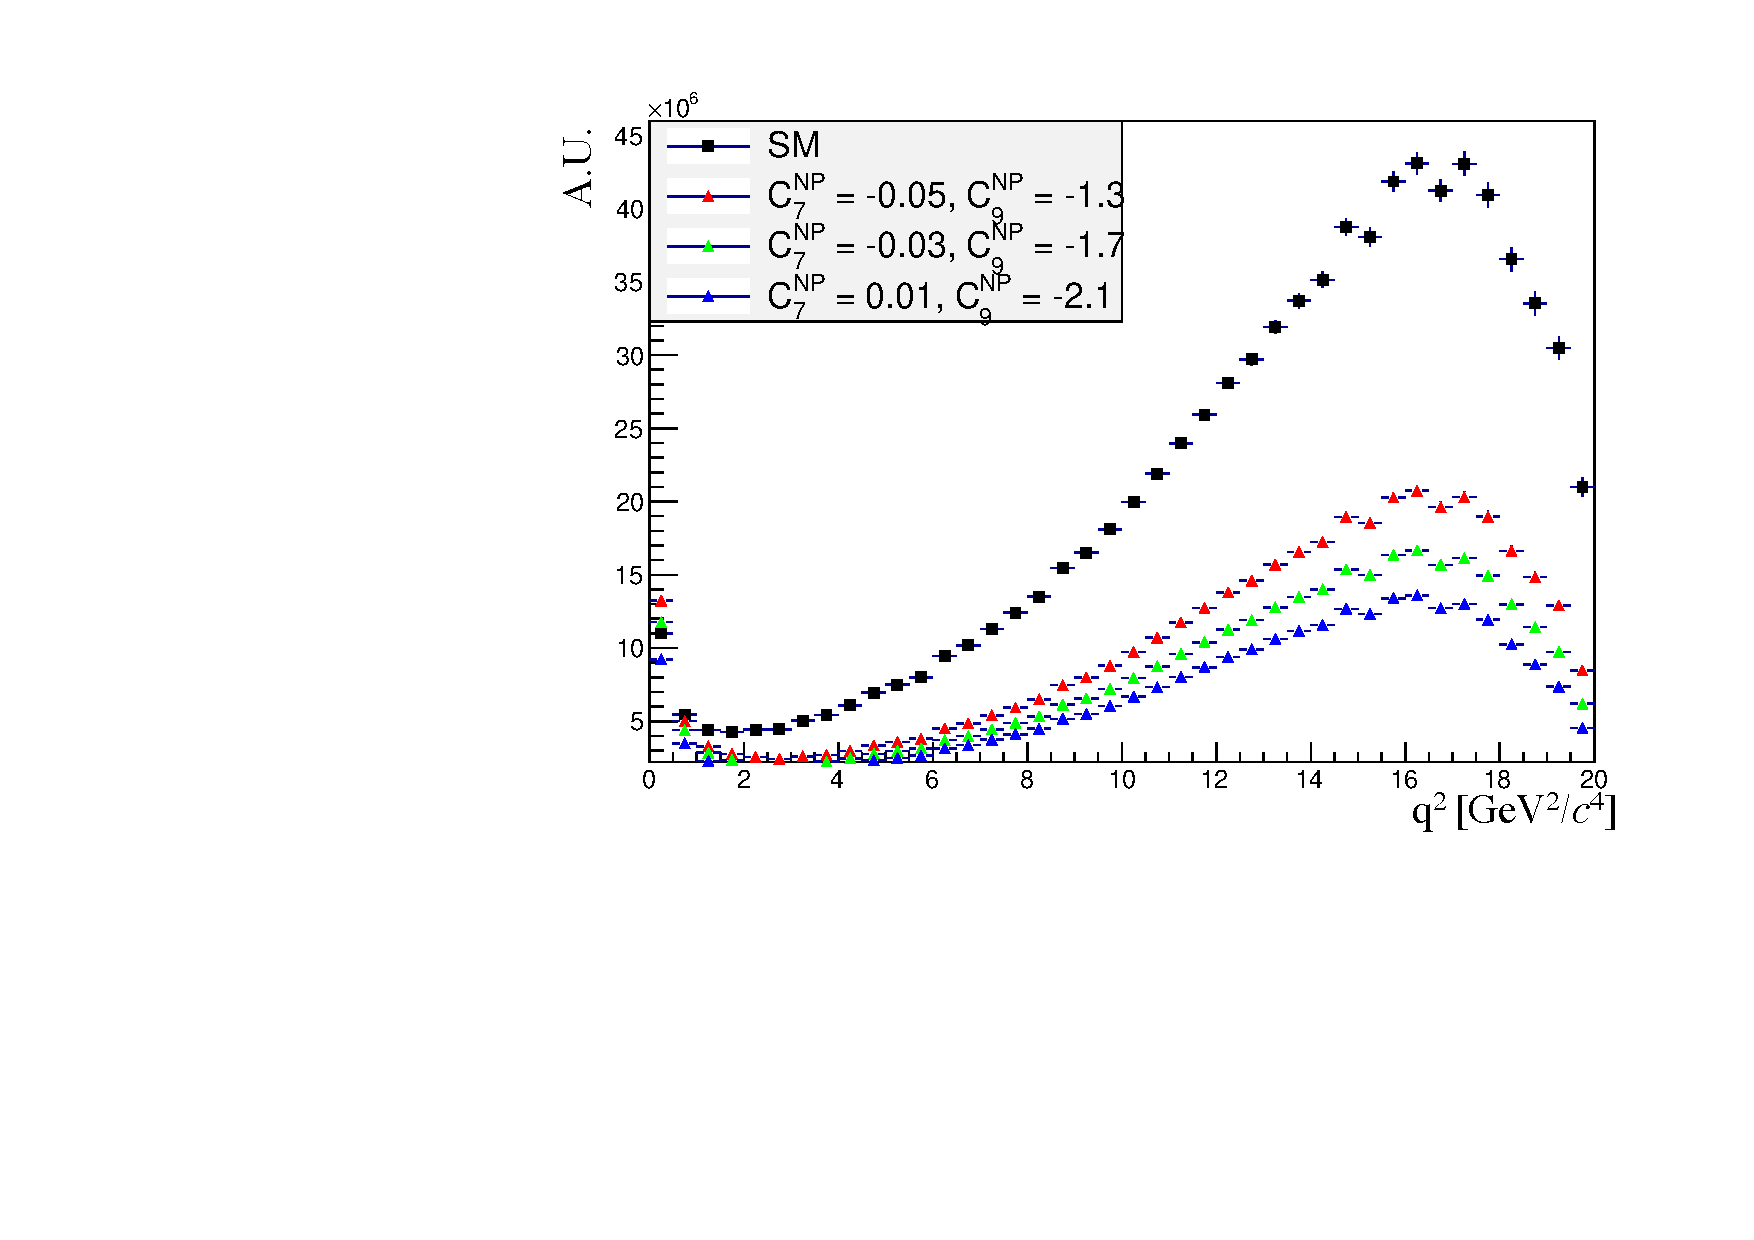
\includegraphics[width=0.8\textwidth]{Lmumu/figs/wilson_q2.pdf}
\caption{The \qsq spectrum of $\Lb\to\Lz\mumu$ simulated events weighted with models embedding different sets of Wilson coefficients.
The black distribution corresponds to the weights used to calculate nominal efficiencies.}
\label{fig:wilson_q2}
\end{figure}
Figure~\ref{fig:wilson_q2} shows \qsq spectra
obtained by weighting the simulation for a model embedding the default and three modified sets
of Wilson coefficients. The values used, reported on the plot legend, are inspired
to maintain compatibility with the recent LHCb measurement of the $P'_5$ observable~\cite{Descotes-Genon:2013wba}.
The biggest effect is observed in the very low \qsq region, below 2~\gevgevcccc, where the efficiency can change
by up to 7\%, while it changes 3 -- 4\% between 3 and 4~\gevgevcccc~and 2 -- 3\% in the rest of the spectrum.
As this analysis is performed under the hypothesis that the decays are described by the SM,
these values are given for completeness but are not added 
as systematic uncertainties. 

%\begin{figure}
%\centering
%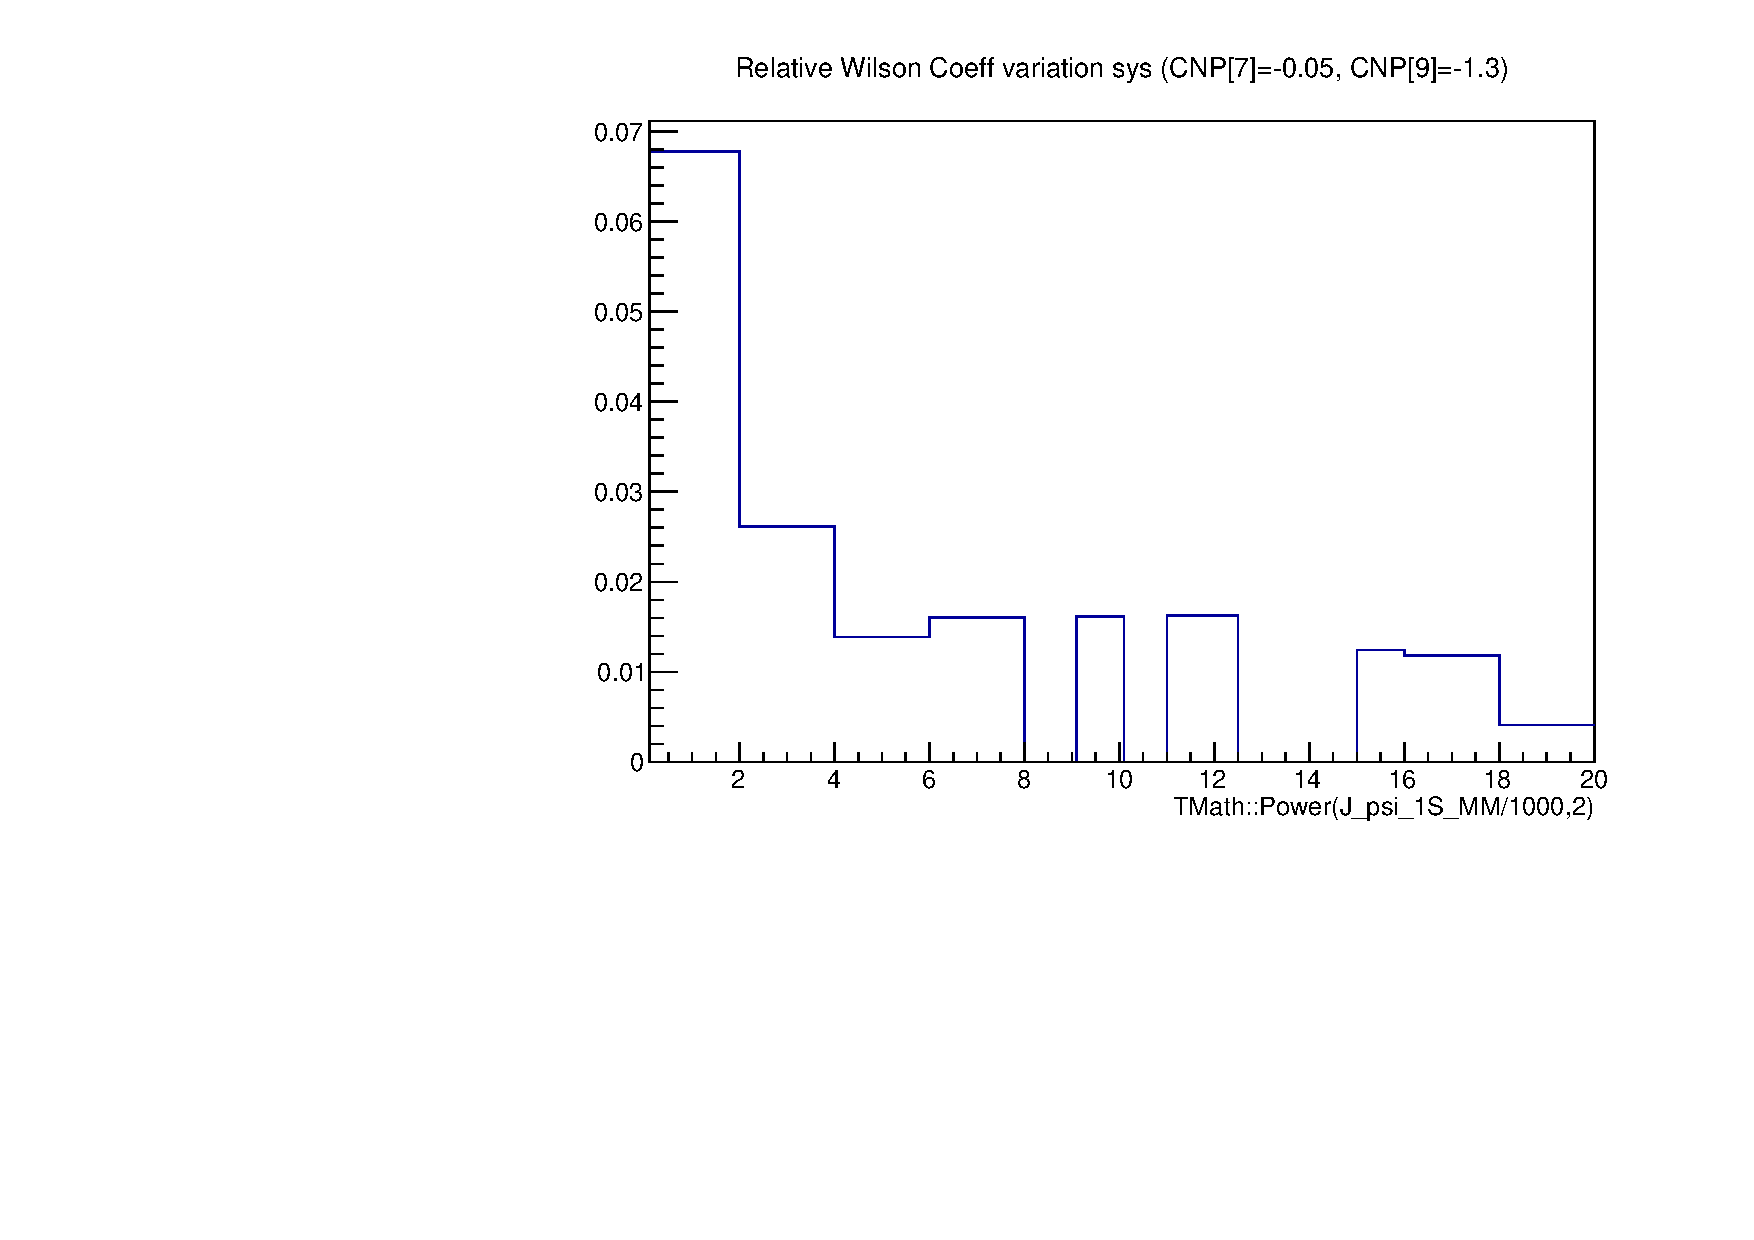
\includegraphics[width=0.48\textwidth]{Lmumu/figs/rel_wilson1_sysAll.pdf}
%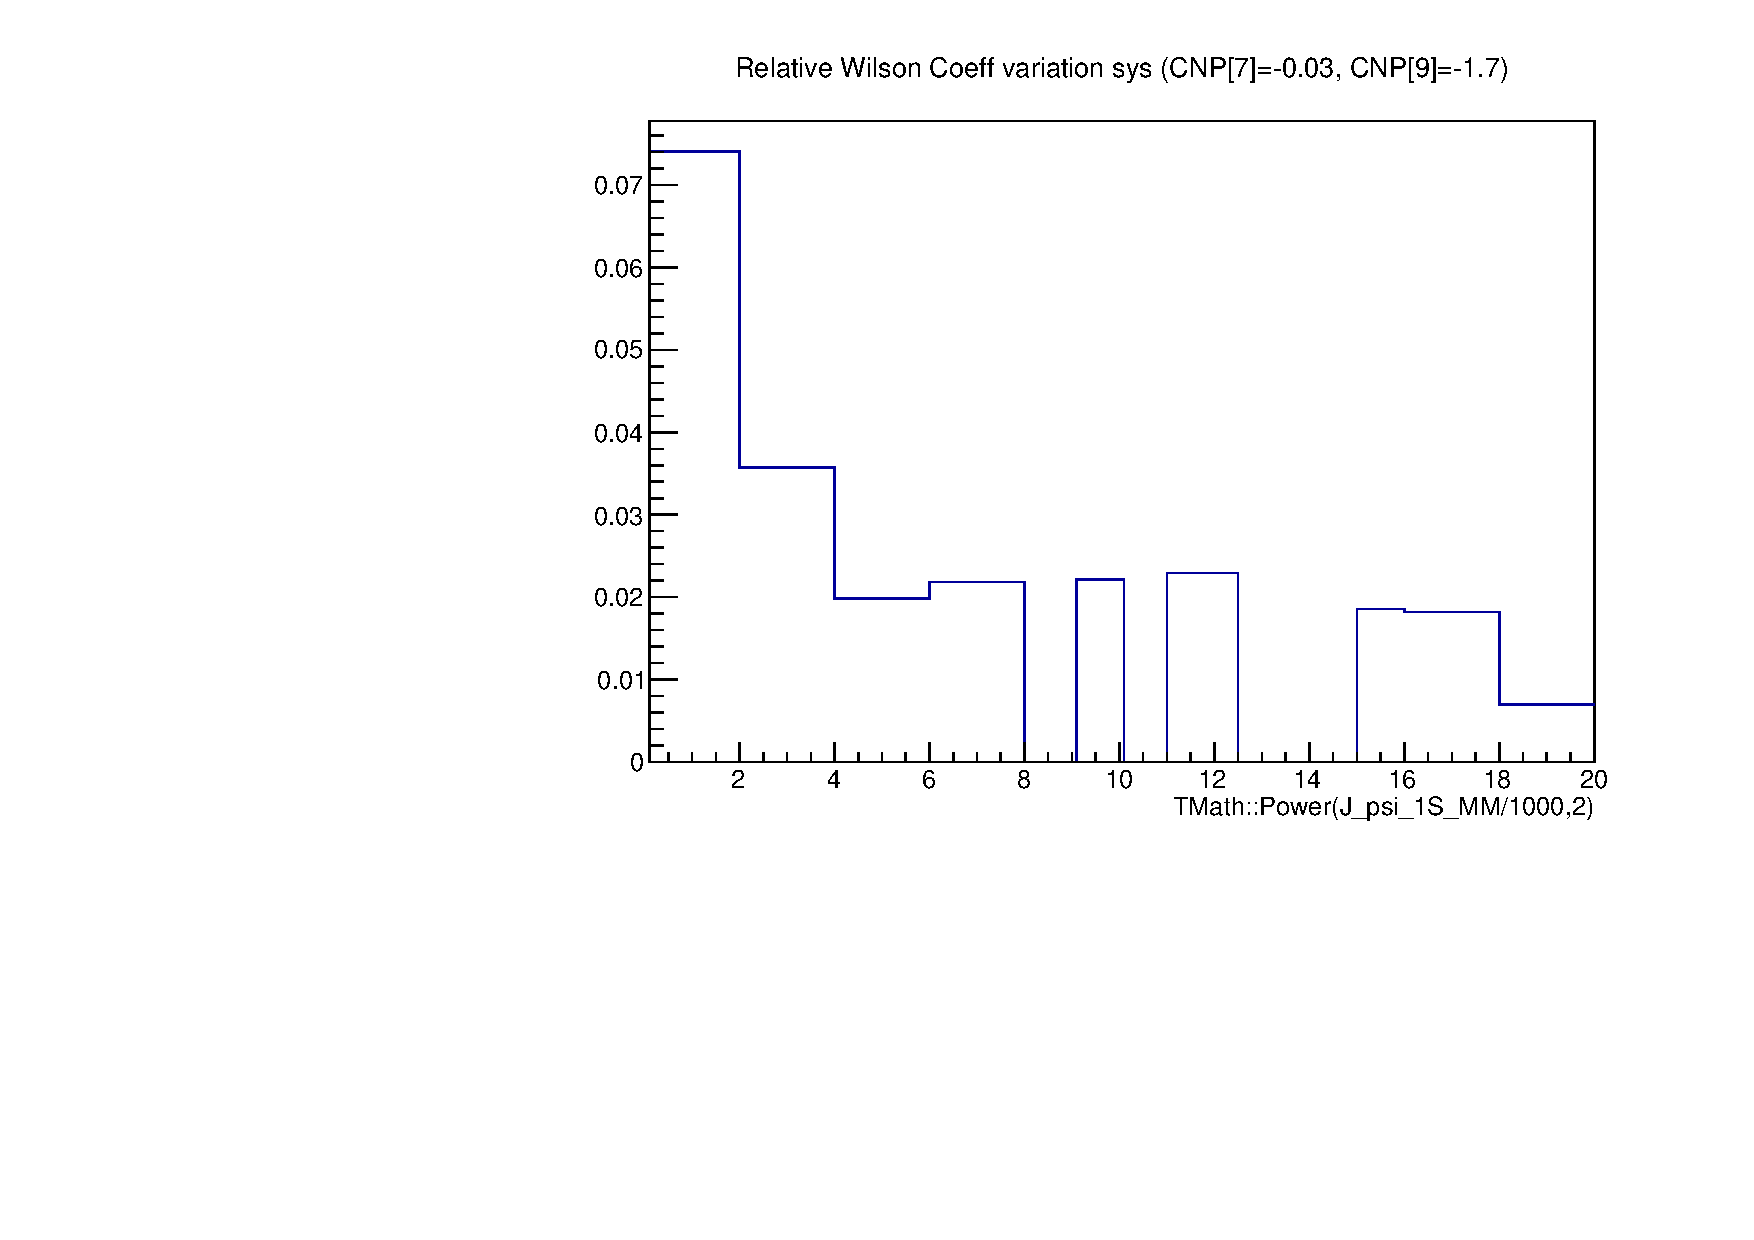
\includegraphics[width=0.48\textwidth]{Lmumu/figs/rel_wilson2_sysAll.pdf} \\
%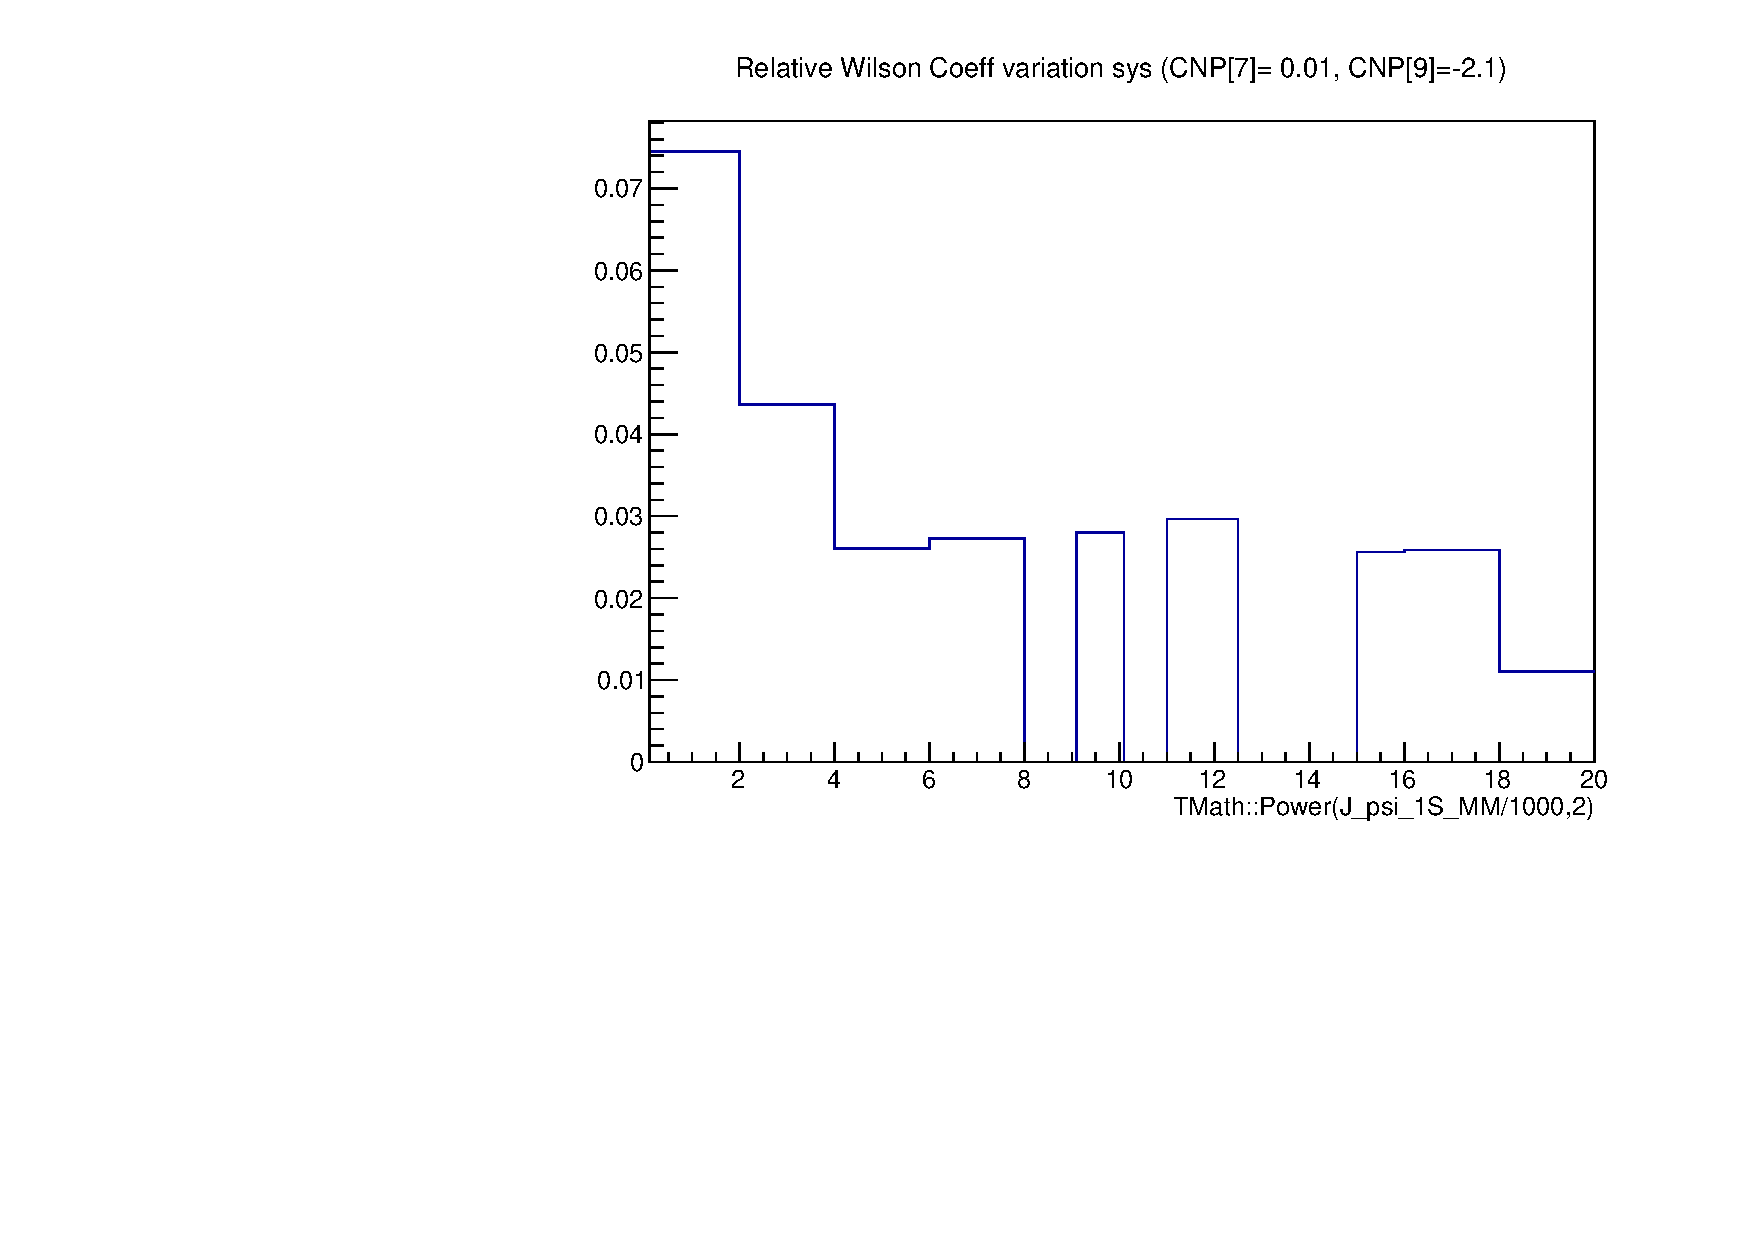
\includegraphics[width=0.48\textwidth]{Lmumu/figs/rel_wilson3_sysAll.pdf}
%\caption{Relative effect of different Wilson Coefficients sets on the total efficiency in bins of \qsq.}
%\label{fig:wilson_diff}
%\end{figure}

\subsubsection{Simulation statistics}

The limited statistics of the simulated samples used to determine the efficiencies is considered 
as a source of systematic uncertainty.
While it is not the dominant source, its size is not completely negligible, 
therefore, when reporting efficiency values, the statistical uncertainty due to the  
rare and resonant channels is always considered. 
%While it would be useful to treat part from normalisation channel separately due to the correlation 
%across \qsq bins, given its size we decide to suppress it as in final presentation its effect is hard to see.

\subsubsection{Production polarisation and decay structure}
\label{sec:BRpolsys}

One of the main unknowns that affects the determination of the efficiencies, is the angular structure of
the decays and the related production polarisation, which is a parameter of the model.
%The normalisation decay $\Lb\to\jpsi\Lz$ is also re-weighted and $\Lb\to\Lz\mumu$ is
%distributed according to the model described in appendix \ref{ap:LbLmumuAngular}.
%
To assess the systematic uncertainty due to the knowledge of the production polarisation for $\Lb\to\Lz\mumu$ decays
the polarisation parameter in the model is varied by one standard deviation from the central value of the
most recent LHCb measurement, $P_b = 0.06 \pm 0.09$~\cite{Aaij:2013oxa}. The full observed difference is
taken as systematic uncertainty. To assess the systematic uncertainty due to the decay structure,
an alternative set of form factors is used based on lattice QCD calculations~\cite{Detmold:2012vy}. 
The two models are compared and the full difference is taken as systematic uncertainty.
%
In total this results in an uncertainty of \mbox{$\sim1.3\%$} for long candidates and \mbox{$\sim0.6\%$} for downstream
candidates, mostly coming from the knowledge of the production polarisation.

\subsubsection{\Lb lifetime}

The \Lb lifetime is known with limited precision. For the evaluation of efficiencies the
world average value, $1.482\pm0.030$~ps$^{-1}$~\cite{Aaij:2013oha}, is used. This is
varied by one standard deviation from the measured value to assess the systematic uncertainty.
Only the case where both signal and normalisation channels are varied in the same direction are considered.
The largest difference from the default lifetime case is taken as the systematic uncertainty,
which is found to vary from $\sim 0.4\%$ at low-\qsq to $\sim 0.1\%$ at high-\qsq.
%We do not attempt to separate out part correlated amongst \qsq bins. This source does not affect
%geometric acceptance, which is defined purely by requirements on angles of each muon with respect to
%beam axis.

\subsubsection{Downstream candidates reconstruction efficiency}

%In the LHCb detector, \Lz can be reconstructed using long or downstream tracks. The distinction is mainly
%driven by the geometry of the detector. A potential issue is that fraction of \Lz reconstructed
%from long tracks and downstream tracks does not fully agree with simulation. For $\Lb\to\jpsi\Lz$
%decay we determine on data that $(26.44 \pm 0.70)$\% of \Lz candidates are reconstructed from long tracks.
%On contrary in simulation of the same decay, only $21.15\pm0.24$\% of candidates are reconstructed
%from long tracks. The same ratio on phase space simulation of $\Lb\to\Lz\mumu$ is $21.54\pm0.14$\%
%(integrated over \qsq). From this we conclude that this ratio is expected to be similar in the two samples and
%that simulation does not fully match data.

Other analysis in LHCb using particles reconstructed from downstream tracks showed that
the efficiency for these candidates is not perfectly simulated.
For example, Fig.~\ref{KS_vtxeff} shows the ratio between the reconstruction efficiency for downstream candidates
in data and simulation found analysing \KS events~\cite{Blake:1631348}. This effect is not
yet fully understood and is currently under study. It seems to be mainly due to a poor simulation
of the vertexing efficiency for downstream tracks.
%
%
However, as the analysis is performed separately for downstream and long candidates and efficiencies are calculated separately, 
the effect of this mis-modelling, present in both the rare and resonant channels, largely cancels in their ratio.
Nevertheless, a systematic uncertainty is assessed by re-weighting simulated candidates 
by the efficiency ratio between data and simulation found for \KS as a function of its momentum (see Fig.~\ref{KS_vtxeff}). 
The efficiencies obtained using the weighted and unweighted simulation are compared and the full difference is taken as the systematic uncertainty. 
As the discrepancy shows little dependence on momentum, dependencies due to the different momentum 
distributions of \Lz and \KS are assumed to be negligible. This results in a systematic uncertainty for downstream candidates
of $\sim 0.4\%$ at low-\qsq and $\sim 1.2\%$ at high-\qsq.

\begin{figure}
\centering
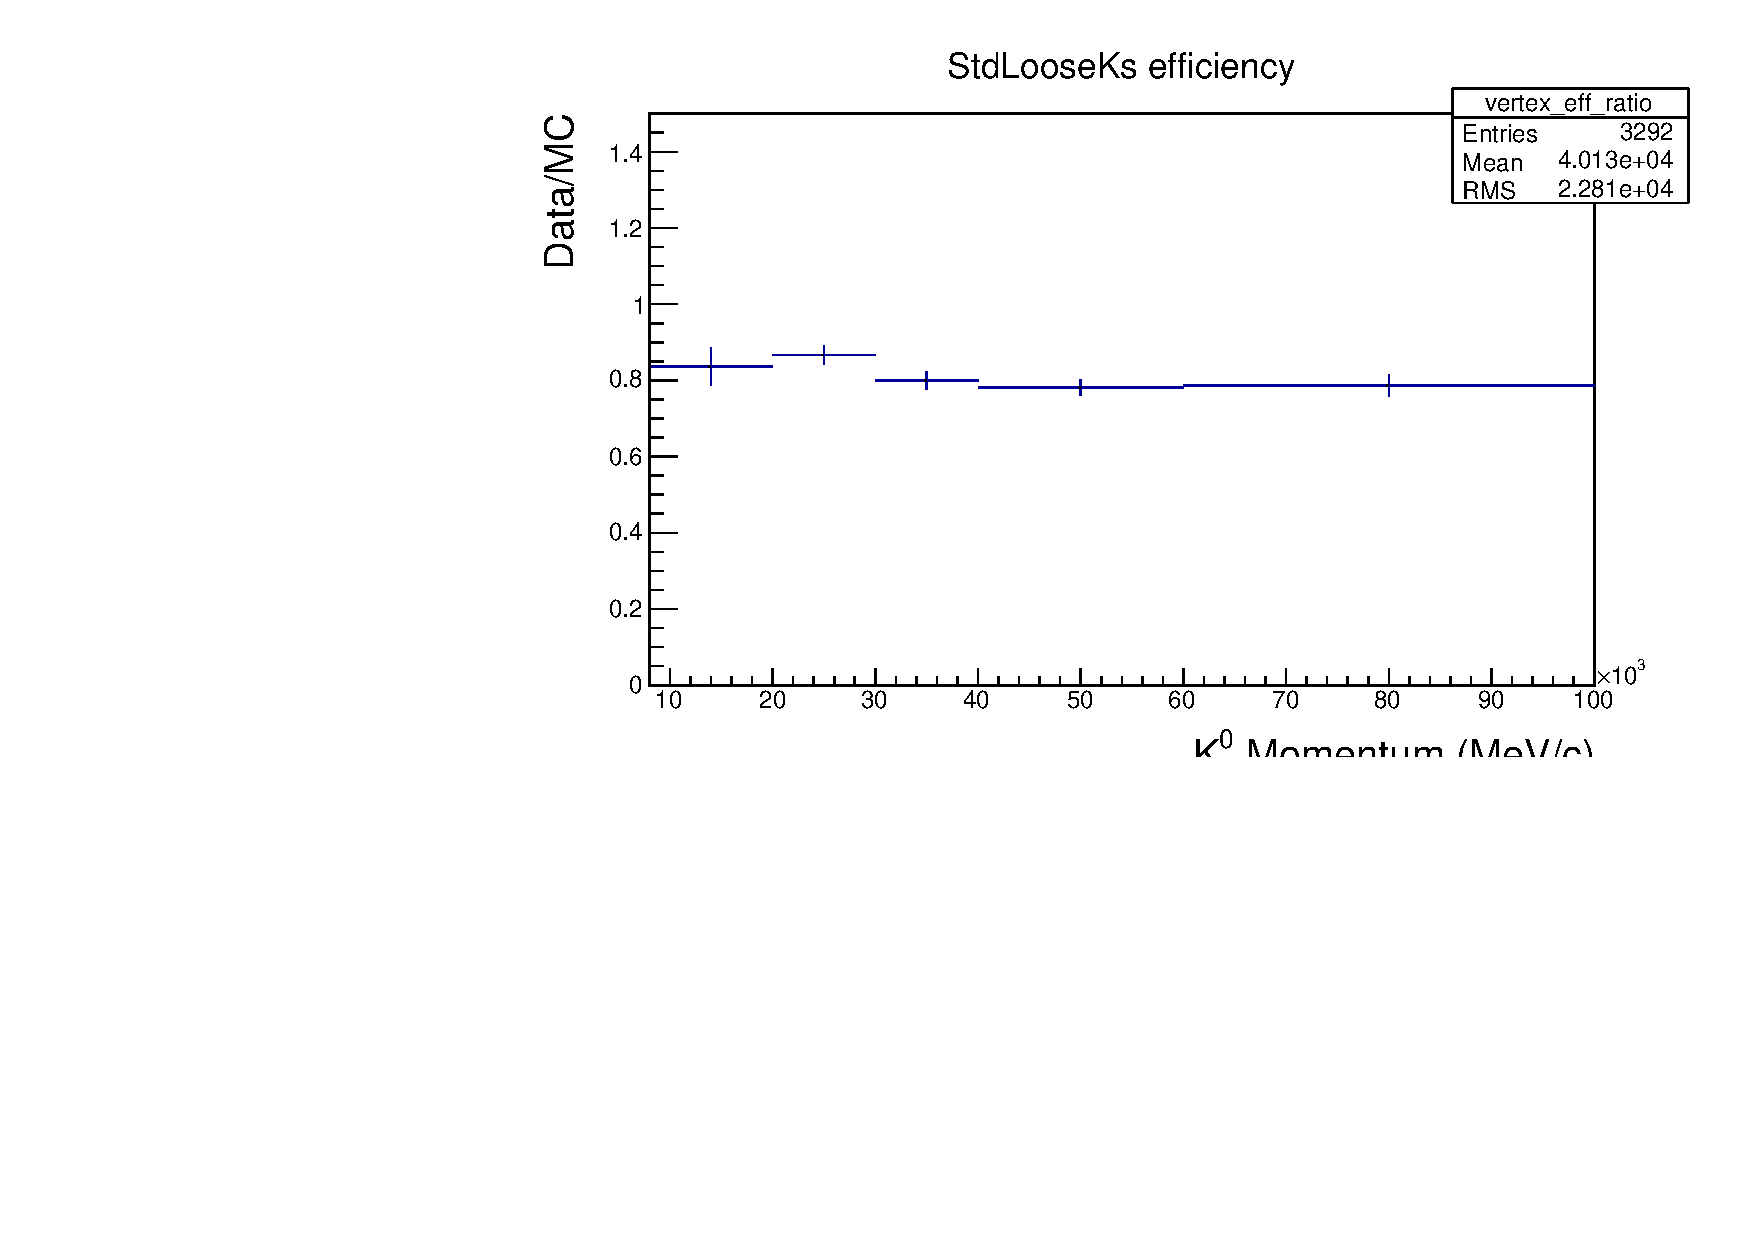
\includegraphics[width=0.8\textwidth]{Lmumu/figs/DDvtx_eff_POwen.pdf}
\caption{Ratio of reconstruction efficiency in data and simulation found using \KS events~\cite{Blake:1631348}.}
\label{KS_vtxeff}
\end{figure}

\subsubsection{Data-simulation discrepancies}

The simulation used to calculate the efficiencies is weighted to 
improve its description of data as described in Sec.~\ref{sec:kinWeight}.
The influence of this procedure on the efficiency determination is checked by comparing values obtained with
and without re-weighting. The effect is negligible with respect to other systematics considered.
%After the kinematical re-weighting there could still be some data-simulation discrepancies.
%In particular the PID variables, used in the Neural Networks, are not perfectly described in the MC.
%We checked if this could be a source of systematics by comparing sideband subtracted data Monte Carlo re-weighted for the
%\Lb kinematics and extracting a further weight to match the PID variable.
%Figure \ref{fig:PIDmysys} shows the difference between the efficiency calculated with and without the further PID weight.
%In all \qsq bins the difference is always compativle with zero within one sigma and therefore we do not add any further systematic
%due to the PIDmu variable modelling.

%\begin{figure}
%\centering
%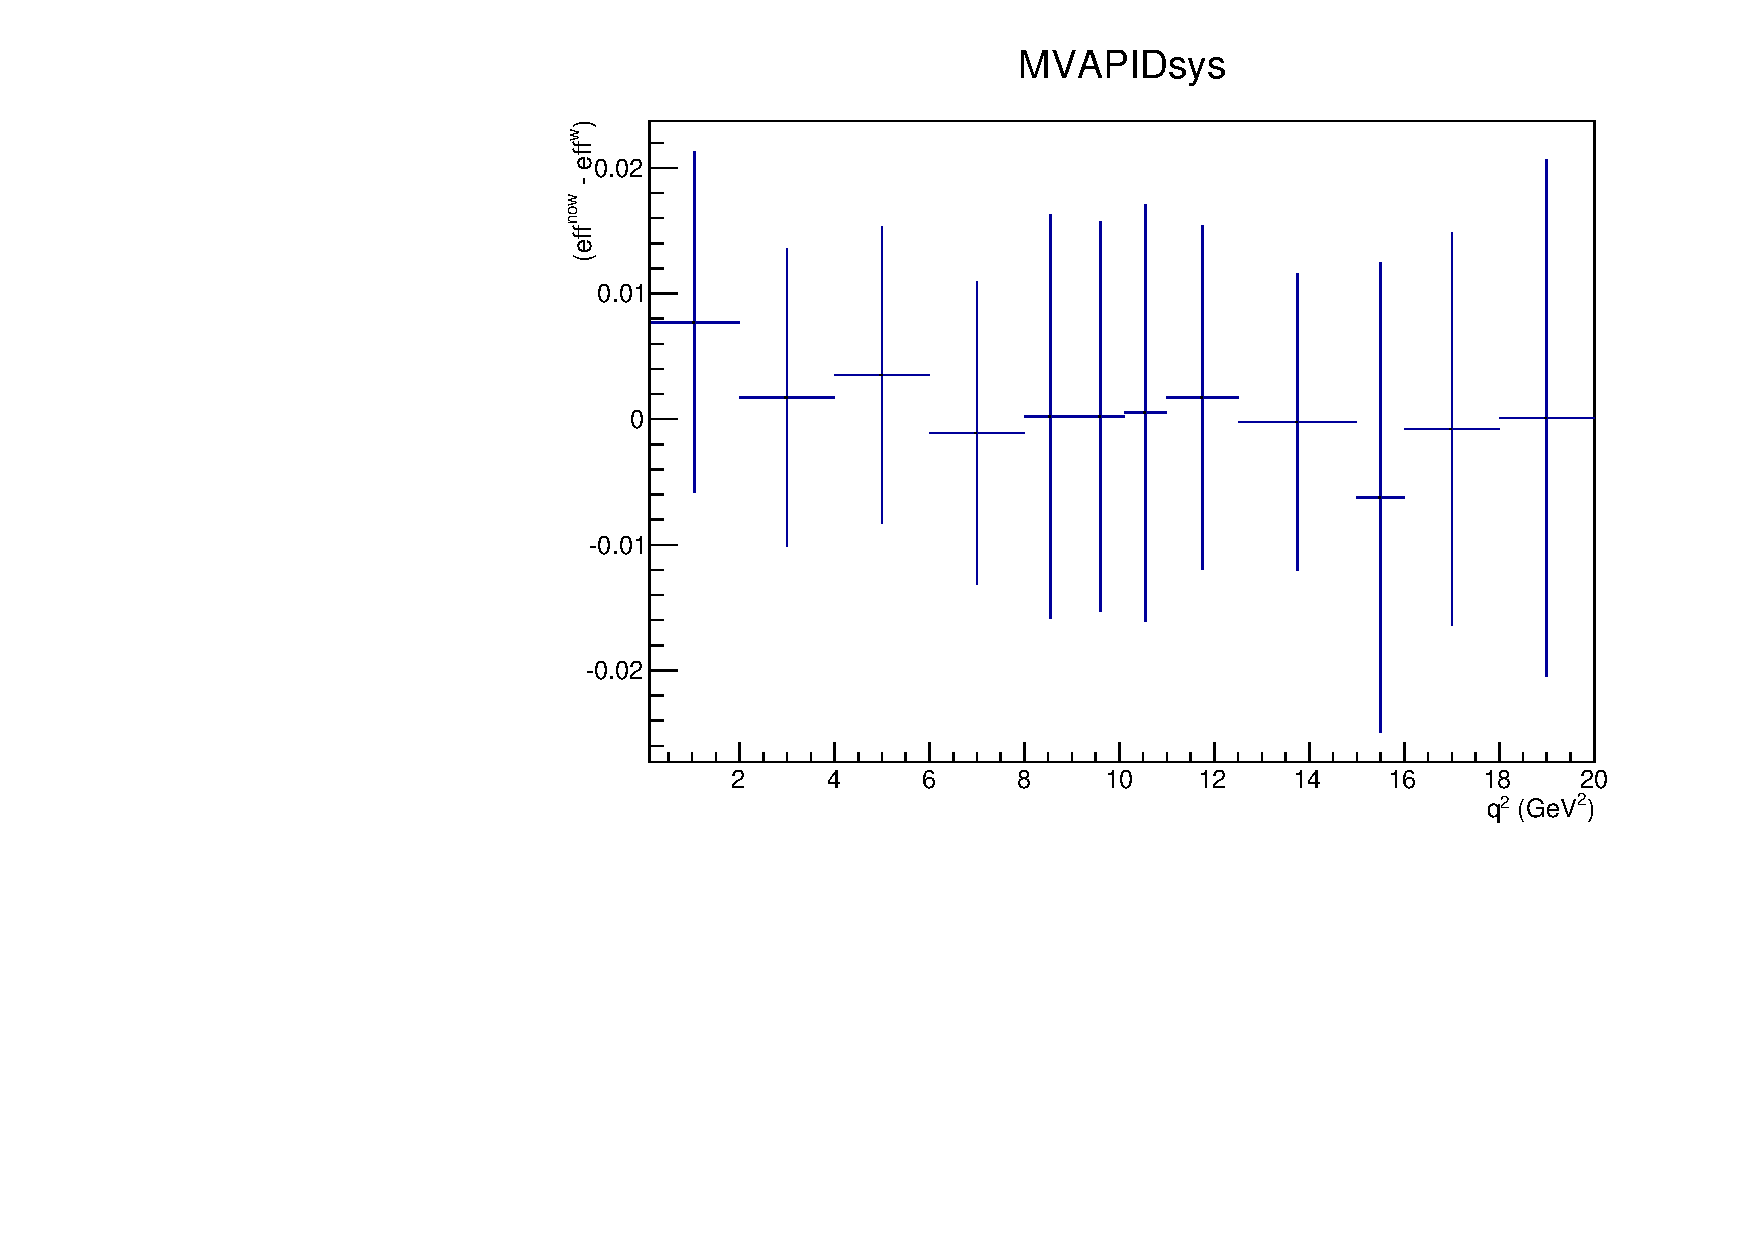
\includegraphics[width=0.6\textwidth]{Lmumu/figs/PIDmu_sys.pdf}
%\caption{Difference between the efficiency calculated with and without the weight to match the PIDmu distributions
%in data and MC as a function of \qsq.}
%\label{fig:PIDmysys}
%\end{figure}


\section{Differential branching fraction extraction}
\label{sec:Lb_BRsummary}

In this section the differential branching fraction of the $\Lb\to\Lz\mumu$ decay is calculated 
relative to the $\Lb\ra\jpsi\Lz$ channel as a function of \qsq.
The values are directly obtained from the fit to the rare sample by parameterising
the downstream and long yields with the following formula:
%
\begin{equation}
N(\Lz\mumu)_{k}  = \left[ \frac{\mathrm{d}\mathcal{B}(\Lz\mumu)/\mathrm{d}\qsq}{\mathcal{B}(\jpsi\Lz)} \right]  \cdot
N(\jpsi\Lz)_{k} \cdot \varepsilon^{\mathrm{rel}}_{k} \cdot \frac {\Delta\qsq} { \mathcal{B}(\jpsi\to\mumu) },
\label{eq:ield_from_BR}
\end{equation}
\noindent
where $k = $(LL,DD), $\Delta\qsq$ is the width of the \qsq interval, 
\mbox{$\mathcal{B}(\jpsi\to\mumu) =$} ($5.93 \pm 0.06)\cdot 10^{-2}$~\cite{PDG2014} and the only free parameter
is the relative branching fraction ratio. Table~\ref{tab:Lb_effSummary} summarises the total relative efficiencies, 
$\varepsilon^{\rm rel}$, for downstream and long candidates together with their correlated and uncorrelated uncertainties, 
where the correlation is intended between the downstream and long samples. In the table the uncorrelated uncertainty 
corresponds to the total systematic uncertainty on the efficiency determination.
The correlated uncertainty is given as a percentage since it can be applied to either downstream or long candidates,  
or their combination. This includes the PDF systematic described in Sec.~\ref{sec:Lb_yield_sys} and the systematic 
due to the uncertainty on the $\jpsi\to\mumu$ branching fraction.

\begin{table}
\centering
\caption{Absolute values of the total relative efficiency of $\Lb\to\Lz\mu\mu$ with respect 
to $\Lb\to\jpsi\Lz$ and the absolute value of the uncorrelated uncertainty ($\sigma_{uncorr}^{k}$), 
together with percent values of the correlated uncertainty ($\sigma_{corr}$), where $k = $(LL,DD). }
\begin{tabular}{$l^c^c^c^c^c}
\rowstyle{\bfseries}
\boldmath{\qsq [\gevgevcccc]}	 & Eff. (DD) 	 &  \boldmath{$\sigma_{uncorr}^{\rm DD}$}	 & Eff. (LL)  &	 \boldmath{$\sigma_{uncorr}^{\rm LL}$} 	 & \boldmath{$\sigma_{corr}$} \\
\hline
\phantom{x}0.1 -- 2.0\phantom{x}    &  0.694  &  0.058  &  1.136  &  0.066  &  1.0\%    \\
\phantom{x}2.0 -- 4.0\phantom{x}    &  0.693  &  0.027  &  0.907  &  0.047  &  2.7\%    \\
\phantom{x}4.0 -- 6.0\phantom{x}    &  0.699  &  0.018  &  0.964  &  0.044  &  2.7\%    \\
\phantom{x}6.0 -- 8.0\phantom{x}    &  0.733  &  0.020  &  0.953  &  0.048  &  2.7\%    \\

11.0 -- 12.5  &  1.254  &  0.032  &  1.140  &  0.057  &  3.4\%    \\
15.0 -- 16.0  &  1.260  &  0.035  &  1.035  &  0.060  &  3.0\%    \\
16.0 -- 18.0  &  1.163  &  0.029  &  0.997  &  0.048  &  1.7\%    \\
18.0 -- 20.0  &  1.023  &  0.027  &  0.782  &  0.040  &  2.7\%    \\
\hline
\phantom{x}1.1 -- 6.0\phantom{x}    &  0.696  &  0.032  &  0.950  &  0.058  &  1.0\%    \\
15.0 -- 20.0  &  1.132  &  0.014  &  0.927  &  0.031  &  1.4\%    \\

\end{tabular}
\label{tab:Lb_effSummary}
\end{table}

Figure~\ref{fig:corrDDLLplots} shows the differential branching fraction obtained by fitting 
the downstream and long samples independently, while
%
\begin{figure}
\centering
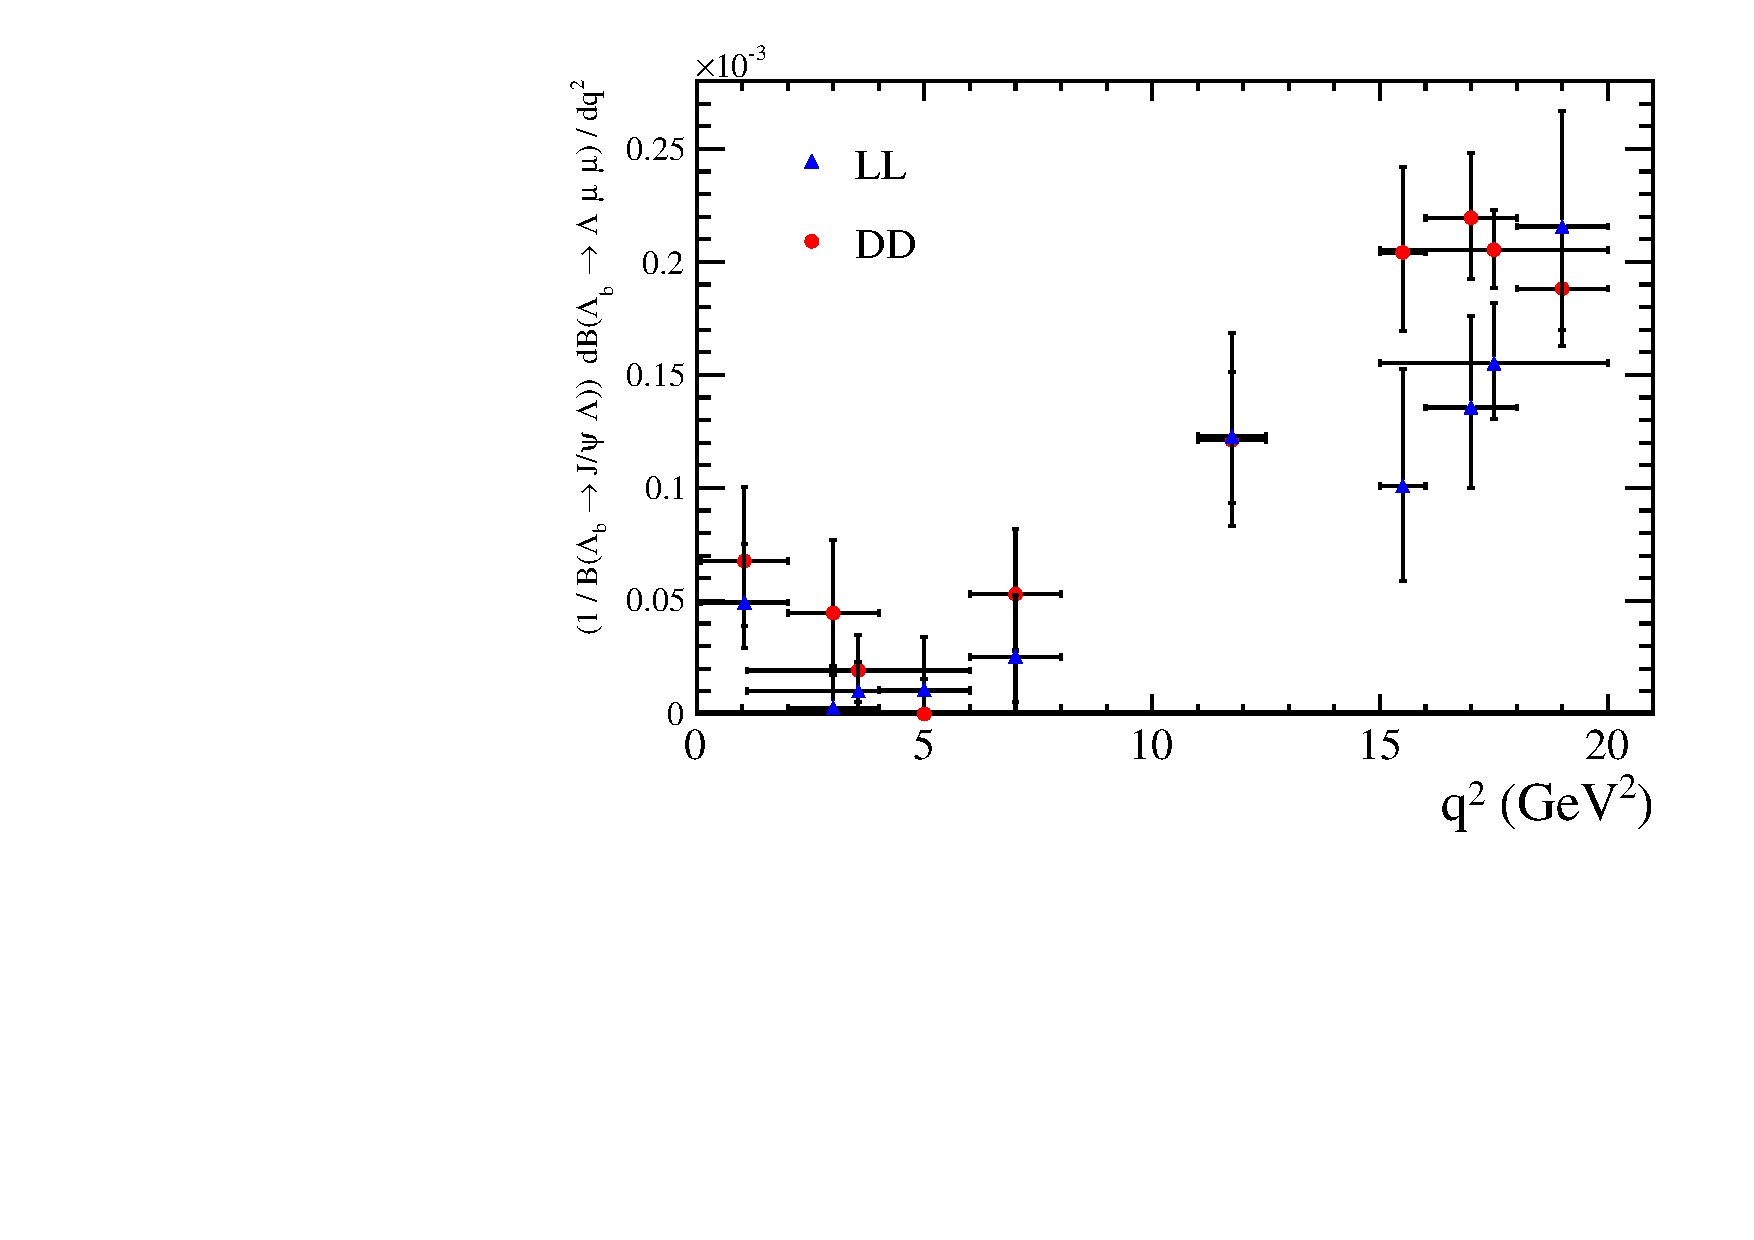
\includegraphics[width=0.8\textwidth]{Lmumu/figs/q2result_both.pdf}
\caption{Measured values of the differential branching fraction of the \mbox{\decay{\Lb}{\Lz\mumu} }
decay relative to the $\Lb\to\jpsi\Lz$ decay as a function of \qsq
obtained fitting the downstream and long samples independently.
Error bars represent the total statistical and systematic uncertainty.}
\label{fig:corrDDLLplots}
\end{figure}
%
%We performed $\chi^2$ consistency test to verify consistency between DD and LL results. We evaluate $\chi^2$ as
%
%\begin{equation}
%\chi^2 = \sum \frac{(Y(DD)_i - Y(LL)_i)^2}{(\sigma_{uncorr}^{LL})^2_i + (\sigma_{uncorr}^{DD})^2_i}
%\end{equation}
%
%where $Y(DD)_i$ and $Y(LL)_i$ are corrected yields for DD and LL events in each bin and $\sigma_{uncorr}^{LL}$($\sigma_{uncorr}^{DD}$) their uncorrelated error,
%including statistical on rare and normalisation channels and uncorrelated systematic error. 
%The result is a $\chi^2$ of 7.0 with 4 degrees of freedom corresponding to a p-value of 0.14.
%
%
%\begin{table}
%\centering
%\renewcommand{\arraystretch}{1.3}
%\begin{tabular}{lc} \hline\hline
%\qsq bin 	 &  $\mathrm{d}\mathcal{B}(\Lz\mumu)/\mathrm{d}\qsq / \mathcal{B}(\jpsi\Lz)$ ($10^{-3}$)\\
%\hline
%\multicolumn{2}{c}{Down-down events} \\ \hline 
%\hline
%
%0.1-2.0  & $    0.0676^{+0.0323}_{-0.0279} \text{(stat)} ^{+0.0055}_{-0.0064} \text{(sys)} ^{+0.0008}_{-0.0008} \text{(norm)} $ \\
%2.0-4.0  & $    0.0447^{+0.0324}_{-0.0275} \text{(stat)} ^{+0.0021}_{-0.0022} \text{(sys)} ^{+0.0005}_{-0.0006} \text{(norm)} $ \\
%4.0-6.0  & $    0.0000^{+0.0155}_{0.0000} \text{(stat)} ^{+0.0000}_{-0.0000} \text{(sys)} ^{+0.0000}_{-0.0000} \text{(norm)} $ \\
%6.0-8.0  & $    0.0530^{+0.0287}_{-0.0248} \text{(stat)} ^{+0.0020}_{-0.0021} \text{(sys)} ^{+0.0007}_{-0.0007} \text{(norm)} $ \\
%11.0-12.5  & $    0.1211^{+0.0300}_{-0.0273} \text{(stat)} ^{+0.0049}_{-0.0053} \text{(sys)} ^{+0.0010}_{-0.0014} \text{(norm)} $ \\
%15.0-16.0  & $    0.2042^{+0.0369}_{-0.0338} \text{(stat)} ^{+0.0082}_{-0.0084} \text{(sys)} ^{+0.0022}_{-0.0022} \text{(norm)} $ \\
%16.0-18.0  & $    0.2196^{+0.0276}_{-0.0260} \text{(stat)} ^{+0.0066}_{-0.0068} \text{(sys)} ^{+0.0023}_{-0.0024} \text{(norm)} $ \\
%18.0-20.0  & $    0.1882^{+0.0259}_{-0.0241} \text{(stat)} ^{+0.0070}_{-0.0071} \text{(sys)} ^{+0.0020}_{-0.0020} \text{(norm)} $ \\
%
%\hline
%1.1-6.0  & $    0.0192^{+0.0157}_{-0.0138} \text{(stat)} ^{+0.0010}_{-0.0011} \text{(sys)} ^{+0.0002}_{-0.0002} \text{(norm)} $ \\
%15.0-20.0  & $    0.2054^{+0.0168}_{-0.0161} \text{(stat)} ^{+0.0039}_{-0.0040} \text{(sys)} ^{+0.0022}_{-0.0022} \text{(norm)} $ \\
%
%\hline
%\multicolumn{2}{c}{Long-long events} \\ \hline
%\hline
%0.1-2.0  & $    0.0493^{+0.0258}_{-0.0200} \text{(stat)} ^{+0.0030}_{-0.0033} \text{(sys)} ^{+0.0009}_{-0.0010} \text{(norm)} $ \\
%2.0-4.0  & $    0.0027^{+0.0186}_{0.0000} \text{(stat)} ^{+0.0002}_{-0.0002} \text{(sys)} ^{+0.0001}_{-0.0001} \text{(norm)} $ \\
%4.0-6.0  & $    0.0107^{+0.0234}_{0.0000} \text{(stat)} ^{+0.0005}_{-0.0006} \text{(sys)} ^{+0.0002}_{-0.0002} \text{(norm)} $ \\
%6.0-8.0  & $    0.0253^{+0.0271}_{-0.0198} \text{(stat)} ^{+0.0014}_{-0.0015} \text{(sys)} ^{+0.0005}_{-0.0005} \text{(norm)} $ \\
%
%11.0-12.5  & $    0.1228^{+0.0451}_{-0.0391} \text{(stat)} ^{+0.0071}_{-0.0076} \text{(sys)} ^{+0.0020}_{-0.0020} \text{(norm)} $ \\
%15.0-16.0  & $    0.1009^{+0.0513}_{-0.0413} \text{(stat)} ^{+0.0063}_{-0.0069} \text{(sys)} ^{+0.0016}_{-0.0017} \text{(norm)} $ \\
%16.0-18.0  & $    0.1356^{+0.0397}_{-0.0348} \text{(stat)} ^{+0.0066}_{-0.0072} \text{(sys)} ^{+0.0022}_{-0.0022} \text{(norm)} $ \\
%18.0-20.0  & $    0.2157^{+0.0497}_{-0.0438} \text{(stat)} ^{+0.0120}_{-0.0129} \text{(sys)} ^{+0.0035}_{-0.0035} \text{(norm)} $ \\
%\hline
%1.1-6.0  & $    0.0101^{+0.0127}_{-0.0099} \text{(stat)} ^{+0.0006}_{-0.0007} \text{(sys)} ^{+0.0002}_{-0.0002} \text{(norm)} $ \\
%15.0-20.0  & $    0.1551^{+0.0260}_{-0.0239} \text{(stat)} ^{+0.0055}_{-0.0058} \text{(sys)} ^{+0.0025}_{-0.0026} \text{(norm)} $ \\
%\hline
%\end{tabular}
%\caption{Values of corrected relative branching fraction for DD and LL events with statistical, correlated and uncorrelated error shown separately. }
%\label{tab:corrDDLL}
%\end{table}
%
%Finally, we combine DD and LL results by a weighted average of the two using the uncorrelated errors as weight, $w_i = 1/(\sigma_i^{uncorr})^2$.
%Using weighted average for each bin the combined result is
%
%\begin{equation}
%y_{combined} = \sum {w_i \cdot Y_i} / \sum {w_i}
%\end{equation}
%
%and its error
%
%\begin{equation}
%\sigma_{combined} = \sqrt{1 / \sum { \sigma_i^{-2} }}.
%\end{equation}
%
%The correlated error is then calculated on the combined yield using the relative values in table \ref{tab:effSummary}.
%
the combined result, obtained fitting both samples simultaneously, is shown in Fig.~\ref{fig:Lb_combBR}.
Measured values are also listed in Tab.~\ref{tab:Lb_combBR}, where the statistical
uncertainty on the rare channel and the total systematic uncertainty are shown separately.
The statistical uncertainty is calculated using the MINOS application of the MINUIT package~\cite{James:1975dr},
which provides an asymmetric interval.
The normalisation and systematic uncertainties are evaluated by adjusting the efficiencies and normalisation yields
up and down by one standard deviation and repeating the fit.
The different efficiencies used translate into a different branching fraction and the full difference with respect 
to the default fit is taken as systematic uncertainty in each direction.


 \begin{figure}[tbph]
 \centering
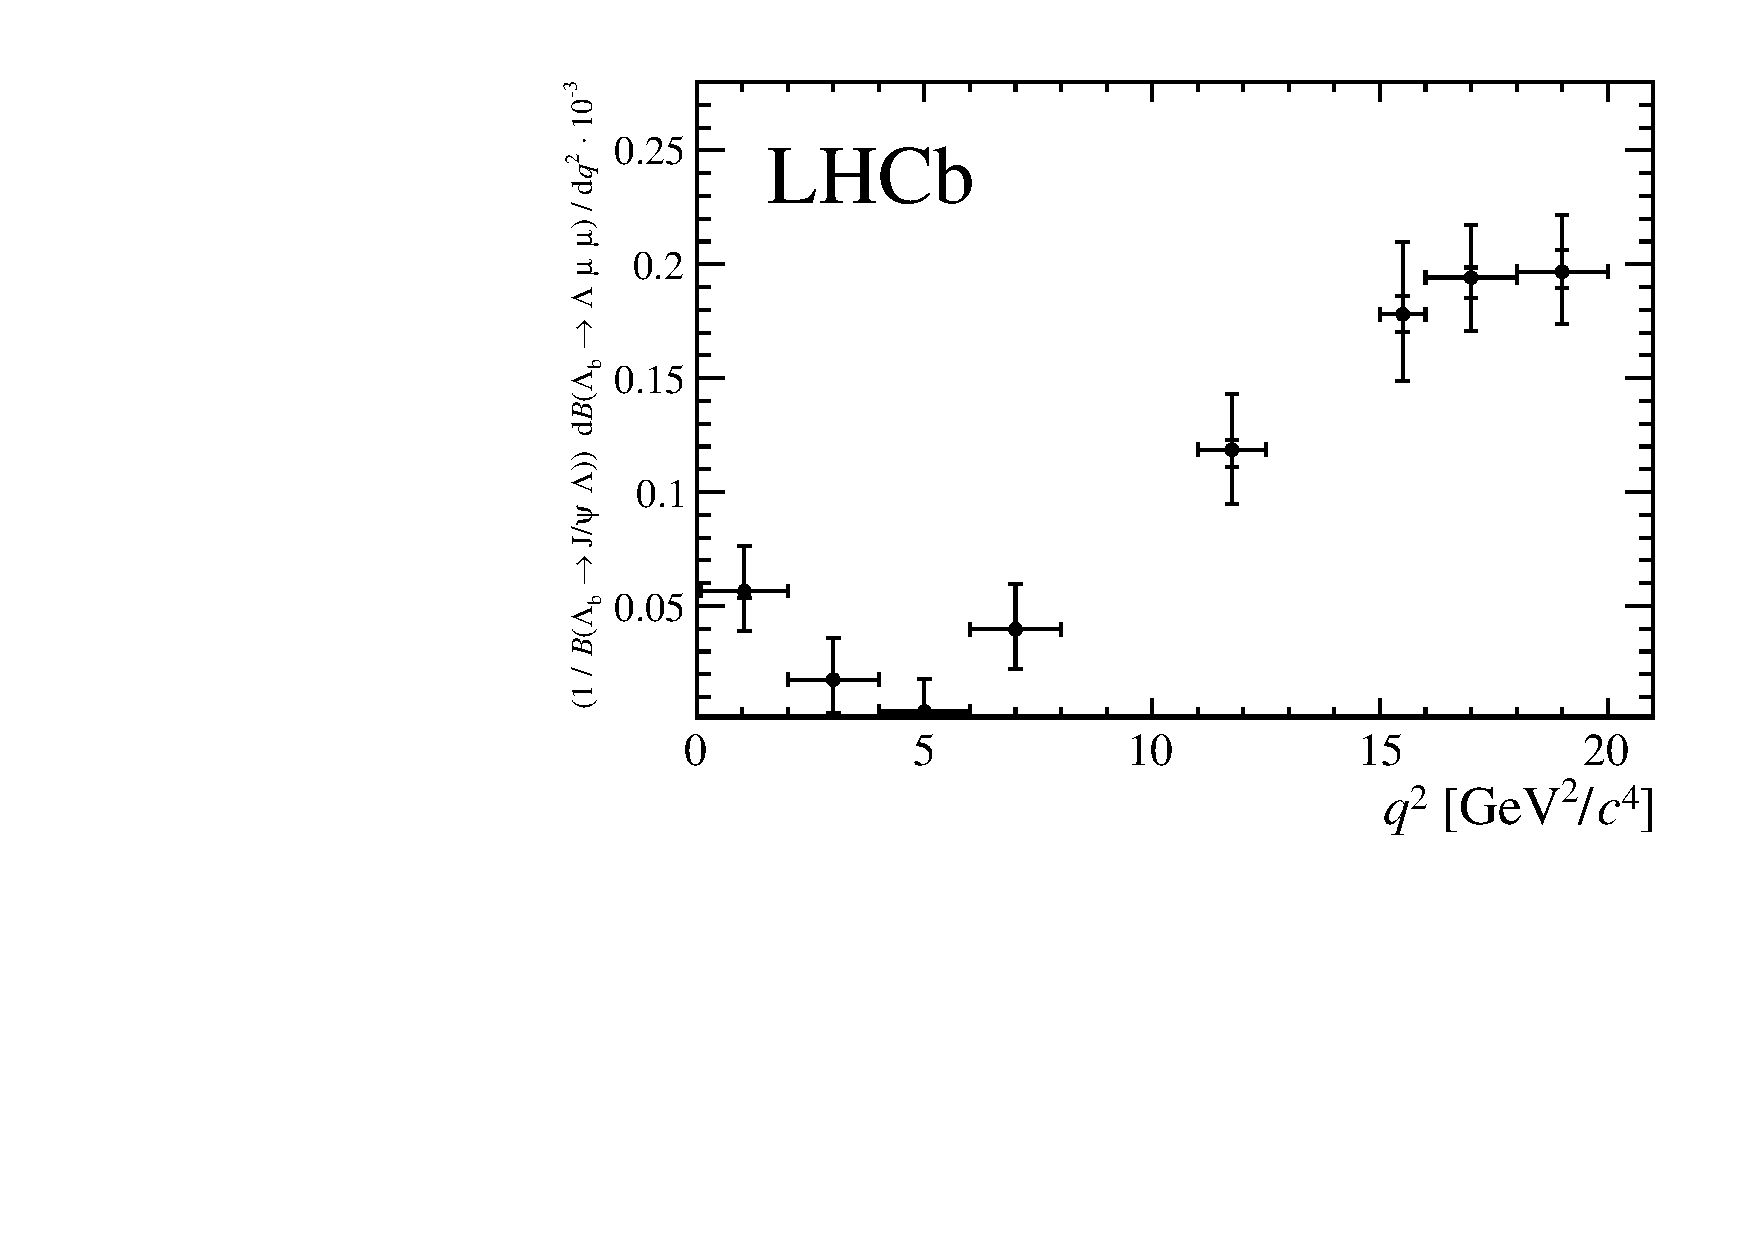
\includegraphics[width=0.8\textwidth]{Lmumu/figs/combined_result_2err.pdf}
\caption{Differential branching fraction of the \decay{\Lb}{\Lz\mumu} decay
  normalised to the \decay{\Lb}{\jpsi\Lz} mode. The inner error bar
  represents the systematic uncertainty and the outer error bar includes
  the statistical uncertainty.} 
   \protect\label{fig:Lb_combBR}
 \end{figure}

\begin{table}
\centering
\renewcommand{\arraystretch}{1.2}
\caption{Measured differential branching fraction of the \decay{\Lb}{\Lz\mumu}
  decay relative to \decay{\Lb}{\jpsi\Lz} decays; uncertainties 
  are statistical and systematic respectively.}
\begin{tabular}{$c^c^c^c^c^c}
\rowstyle{\bfseries}
\boldmath{\qsq [\gevgevcccc]} & &\multicolumn{4}{c}{ $\frac{\deriv\BF(\decay{\Lb}{\Lz\mumu})/\deriv\qsq}{\BF(\decay{\Lb}{\jpsi\Lz})} \cdot 10^{-3} [(\gevgevcccc)^{-1}]$} \\
  
\hline
0.1 -- 2.0   & &0.56 & $^{+0.20}_{-0.17}$ & $^{+0.03}_{-0.03}$ & \\
2.0 -- 4.0   & &0.18 & $^{+0.18}_{-0.15}$ & $^{+0.01}_{-0.01}$ & \\
4.0 -- 6.0   & &0.04 & $^{+0.14}_{-0.04}$ & $^{+0.01}_{-0.01}$ & \\
6.0 -- 8.0   & &0.40 & $^{+0.20}_{-0.17}$ & $^{+0.01}_{-0.02}$ &\\
                                                 
11.0 -- 12.5 & &1.19 & $^{+0.24}_{-0.23}$ & $^{+0.04}_{-0.07}$& \\
15.0 -- 16.0 & &1.78 & $^{+0.31}_{-0.28}$ & $^{+0.08}_{-0.08}$&\\
16.0 -- 18.0 & &1.94 & $^{+0.23}_{-0.22}$ & $^{+0.04}_{-0.09}$&\\
18.0 -- 20.0 & &1.97 & $^{+0.23}_{-0.22}$ & $^{+0.10}_{-0.07}$&\\
              
\hline        
1.1 -- 6.0   & &0.14 & $ ^{+0.10}_{-0.09}$& $^{+0.01}_{-0.01}$&\\
15.0 -- 20.0 & &1.90 & $ ^{+0.14}_{-0.14}$& $^{+0.04}_{-0.06}$&\\
\end{tabular}
\label{tab:Lb_combBR}
\end{table}

Finally, values for the absolute branching fraction of the \decay{\Lb}{\Lz\mumu} decay are obtained by multiplying 
the relative values listed in Tab.~\ref{tab:Lb_combBR} by the branching fraction of the normalisation channel,
$\BF(\decay{\Lb}{\jpsi\Lz})=(6.3\pm1.3)\times10^{-4}$~\cite{PDG2014}.
Values are shown in Fig.~\ref{fig:Lb_absBR} and summarised in Tab.~\ref{tab:Lb_absBR}, where the uncertainty
due to the knowledge of the normalisation channel, which is correlated across \qsq intervals, is shown separately.
The SM predictions on the plot are obtained from Ref.~\cite{Detmold:2012vy}.  

Evidence for the signal in the interval \mbox{$0.1 < \qsq < 2.0$~\gevgevcccc}, where an enhanced yield is expected 
due to the proximity of the photon pole and in the region between the two charmonium resonances is found for the first time. 
The uncertainty on the relative branching fraction is dominated by the size of the available data sample, while,
the uncertainty on the absolute values is dominated by the precision with which the branching 
fraction of the normalisation channel is known.
The measurement is consistent with the theoretical predictions in the high-\qsq region 
but lies below the predictions in the low-\qsq region. Improved predictions published after the publication 
of the LHCb result are reported in Appendix~\ref{app:newpredictions}, where a better agreement is found.

\begin{figure}
\centering
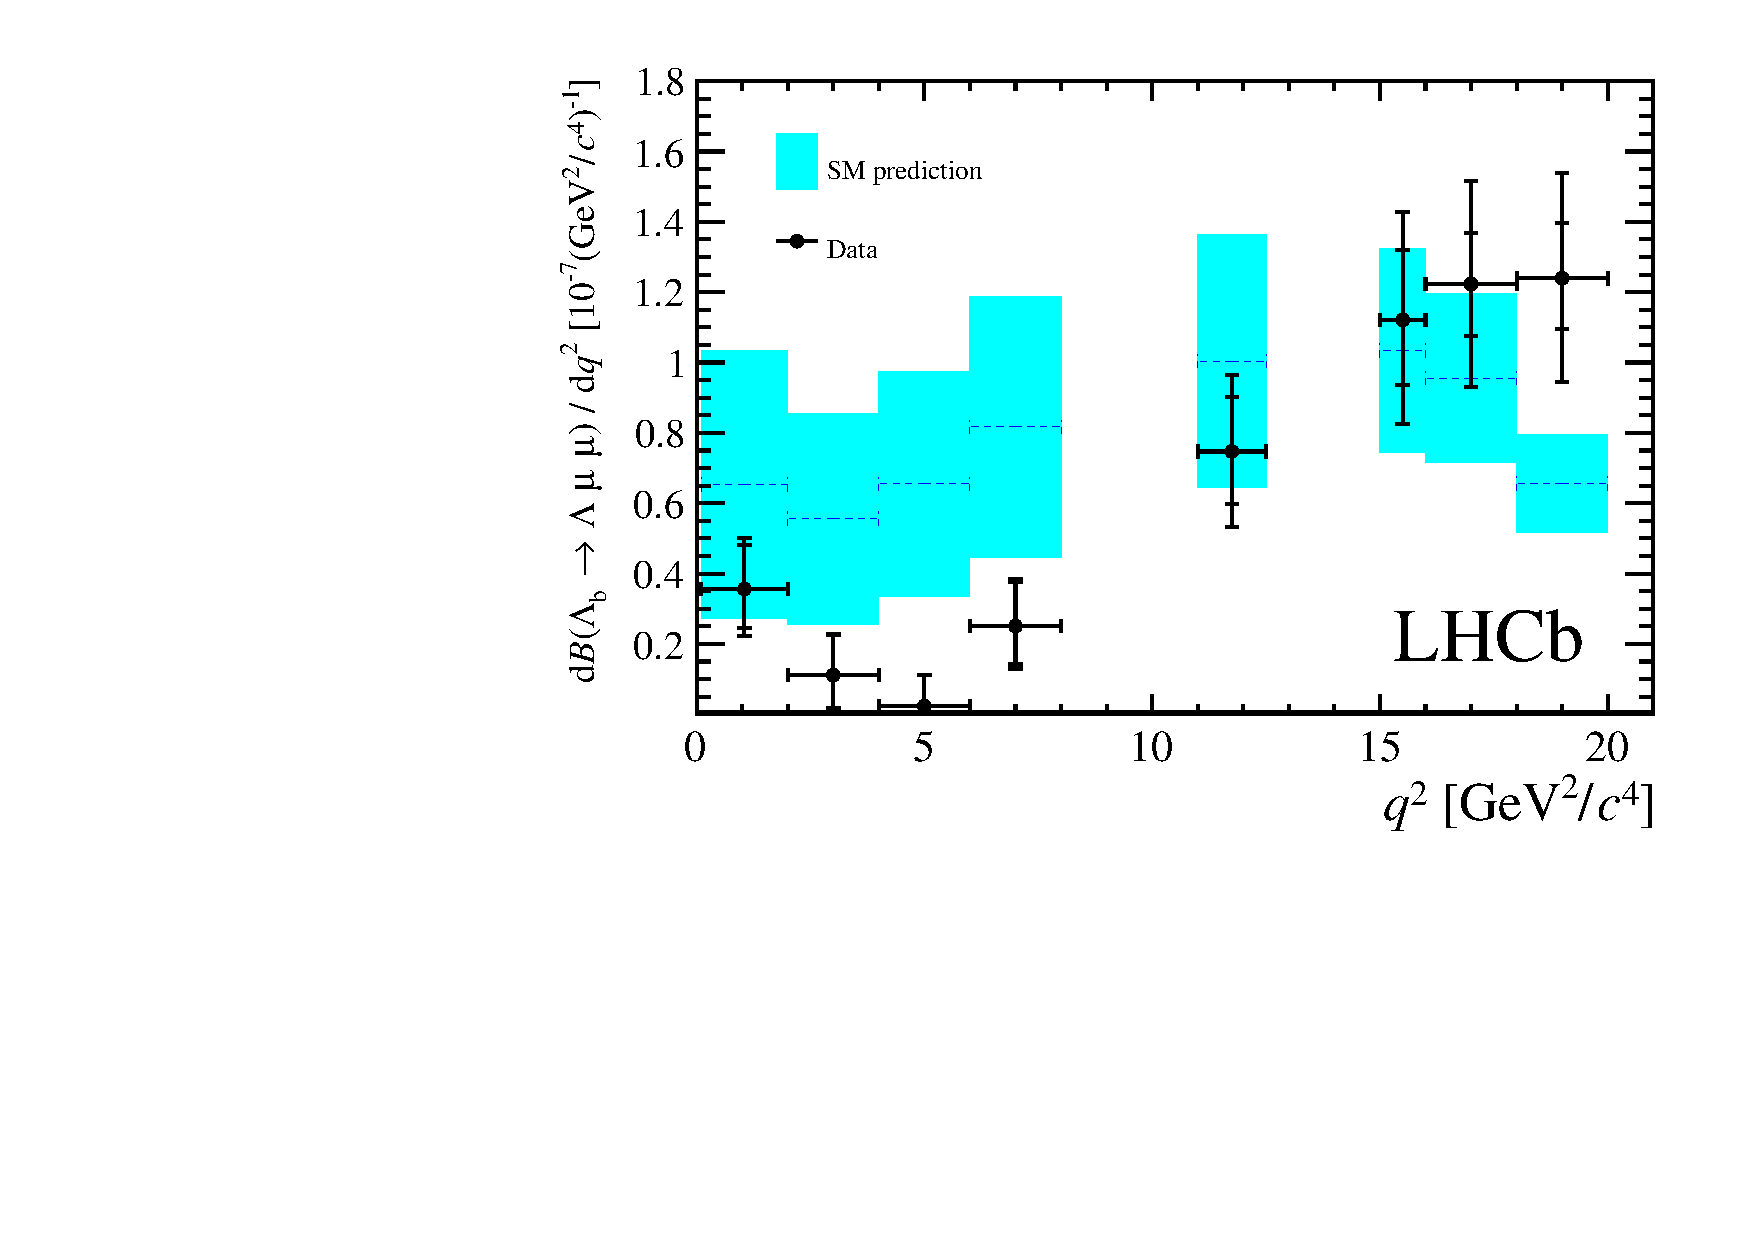
\includegraphics[width=0.8\textwidth]{Lmumu/figs/paper/figure5.pdf}
\caption{Measured \protect\decay{\Lb}{\Lz\mumu} branching
   fraction as a function of \qsq with SM predictions~\cite{Detmold:2012vy} superimposed.  
   The inner error bars represent the total uncertainty on the relative branching
   fraction (statistical and systematic), while the outer error bar also
   includes the uncertainties due to the knowledge of the branching fraction of the
   normalisation mode.}  
\label{fig:Lb_absBR}
\end{figure}

\begin{table}[tbph]
\centering
\renewcommand{\arraystretch}{1.2}
\caption{Measured differential branching fraction of the
  \decay{\Lb}{\Lz\mumu} decay, where the uncertainties are statistical, systematic and
 due to the knowledge of the normalisation mode, \decay{\Lb}{\jpsi\Lz}, respectively.}
\begin{tabular}{$c^c^c^c^c^c^c}
\rowstyle{\bfseries}
  \qsq interval  [\gevgevcccc] & &\multicolumn{5}{c}{$\deriv \BF(\decay{\Lb}{\Lz\mumu})/\deriv\qsq \cdot 10^{-7} [(\gevgevcccc)^{-1}]$} \\
\hline
0.1 -- 2.0    &    &0.36  &  $^{+\,0.12}_{-\,0.11}$   & $^{+\,0.02}_{-\,0.02}$ & $\pm\,0.07$ \\
2.0 -- 4.0    &    &0.11  &  $^{+\,0.12}_{-\,0.09}$   & $^{+\,0.01}_{-\,0.01}$ & $\pm\,0.02$ \\
4.0 -- 6.0    &    &0.02  &  $^{+\,0.09}_{-\,0.00}$   & $^{+\,0.01}_{-\,0.01}$ & $\pm\,0.01$ \\
6.0 -- 8.0    &    &0.25  &  $^{+\,0.12}_{-\,0.11}$   & $^{+\,0.01}_{-\,0.01}$ & $\pm\,0.05$ \\

11.0 -- 12.5  &    &0.75  &  $^{+\,0.15}_{-\,0.14}$   & $^{+\,0.03}_{-\,0.05}$ & $\pm\,0.15$ \\
15.0 -- 16.0  &    &1.12  &  $^{+\,0.19}_{-\,0.18}$   & $^{+\,0.05}_{-\,0.05}$ & $\pm\,0.23$ \\
16.0 -- 18.0  &    &1.22  &  $^{+\,0.14}_{-\,0.14}$   & $^{+\,0.03}_{-\,0.06}$ & $\pm\,0.25$ \\
18.0 -- 20.0  &    &1.24  &  $^{+\,0.14}_{-\,0.14}$   & $^{+\,0.06}_{-\,0.05}$ & $\pm\,0.26$ \\

\hline
1.1 -- 6.0    &    &0.09  &  $^{+\,0.06}_{-\,0.05}$   & $^{+\,0.01}_{-\,0.01}$ & $\pm\,0.02$ \\
15.0 -- 20.0  &    &1.20  &  $^{+\,0.09}_{-\,0.09}$   & $^{+\,0.02}_{-\,0.04}$ & $\pm\,0.25$ \\
 \end{tabular}
\label{tab:Lb_absBR}
\end{table}





\clearpage







